% Chapter 2

\chapter{Background} % Write in your own chapter title
\label{Chapter2}
\lhead{Chapter 2. \emph{Background and Related Work}}

\section{Related Work}

There has been much research done on the task of weather classification. Most works follow the procedure of extracting features and performing classification \citep{bishop1995neural,roser2008classification,serrano2002computationally,gokalp2007scene}.
Some works use low-level features, like colour \citep{szummer1998indoor}, texture \citep{shotton2009textonboost,vailaya2002automatic}. Some works use filters or segmentation \citep{boutell2004learning,shotton2009textonboost} to extract high-level features, such as sky, shadow \citep{lutwo}. Some works use statistical measurement methods \citep{he2014spatial,roser2008classification} to analyse low-level feature distributions.

Generally, the traditional methods follow three basic steps \citep{roser2008classification,yan2009weather}. First, some Regions of Interest (ROIs), for example, sky and shadow,  are extracted from a weather image. Then, histogram descriptors are used to represent the difference between them. Finally, a classifier, e.g., SVM, is built based on the extracted features. 

Most previous works are based on the discriminative model. They extract human recognisable features to classify images. This type of shadow learning depends mainly on the quality of features and human's prior knowledge. An image without prior features or poor features is hard to be classified. Furthermore, the methods require a lot of work on data pre-processing and are not flexible. The approaches depend on structural information to categorise an image into one of the classes. Structural information is concluded from illumination invariant features, like SIFT. However, previous works have limitation on classifying diverse images. It is hard to list all the factors which determinate the weather conditions.

\section{Single-Layer ANNs}

Artificial neurons were introduced as information processing devices more than fifty years ago \citep{mcculloch1943logical}. Following the early work, perceptrons were deployed in layers to do pattern recognition tasks. A lot of resources were invested in the research capability of learning perceptrons theoretically and experimentally. As shown in Figure 2.1, a perceptron computes a weighted summation of its $n$ inputs and then thresholds the result to give a binary output $y$. We can treat $n$ input as an vector with $n$ elements, and represent the vector as either class A(for output +1) or class B(for output -1).
\graphicspath{ {./Figures/} }
\begin{figure}[!htb]
\centering
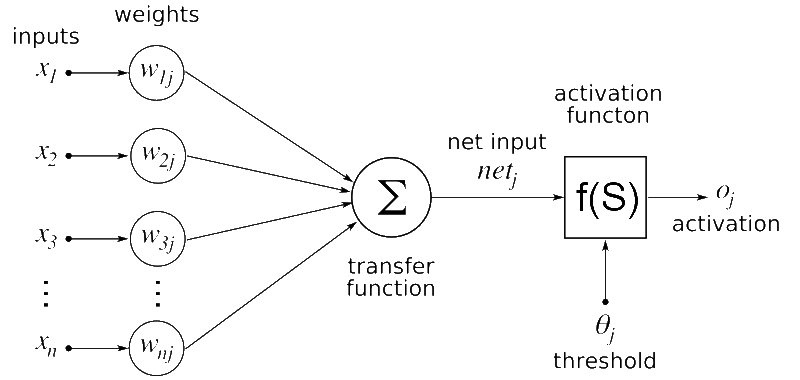
\includegraphics[width=0.8\textwidth]{Figure2-1.png}
\caption{\label{fig:perceptron}Diagram of a perceptron \citep{NeuronFigure1}.}
\end{figure}

Each output is updated according to the equation:
\begin{equation}\label{eq:BasicEq}
y_{i} = f(h_{i}) = f\left(\sum_{j}w_{ij}x_{j}\right)
\end{equation}
where $x_{j}$ is the $j$th input, $y_{i}$ is the $i$th output, and $h_{i}$ is the net input into node. The weight $w_{ij}$ connects the $j$th input and the $i$th output, and the threshold function $f(h)$ is the activation function and usually makes up the form
\begin{equation}\label{eq:FullEq}
f(x) = sign(x) = 
  \begin{cases}
    -1       & \quad h < 0 \\
    1  & \quad h \geq 0\\
  \end{cases}
\end{equation}
and it is plotted out in figure \ref{fig:ThresholdFunc}
\graphicspath{ {./Figures/} }
\begin{figure}[!htb]
\centering
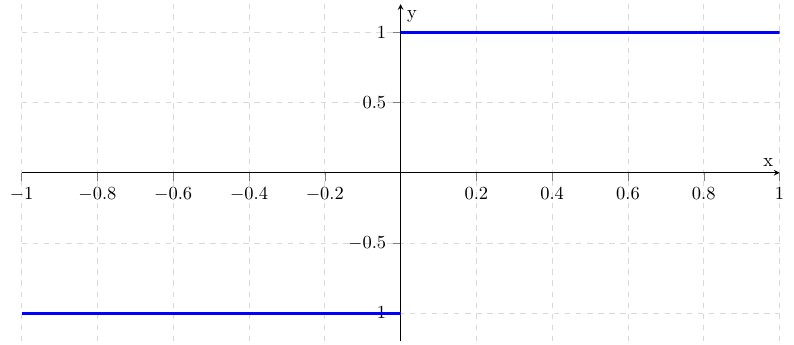
\includegraphics[width=0.4\textwidth]{ThresholdFunc.jpeg}
\caption{\label{fig:ThresholdFunc}Threshold function}
\end{figure}

Besides the threshold function, there are several deterministic action functions.
\begin{itemize}
  \item Linear function 
\begin{equation}\label{eq:LinearFunc}
f(x) = x
\end{equation}

\graphicspath{ {./Figures/} }
\begin{figure}[!htb]
\centering
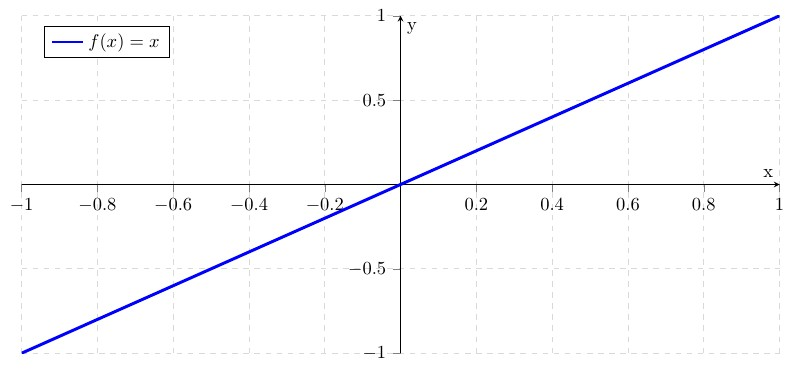
\includegraphics[width=0.4\textwidth]{Linear_function.jpeg}
\caption{\label{fig:LinearFunc}Linear function}
\end{figure}
  
  \item Sigmoid function
\begin{equation}\label{eq:SigmoidFunc}
f(x) = \frac{1}{1+e^{-x}}
\end{equation}

\graphicspath{ {./Figures/} }
\begin{figure}[!htb]
\centering
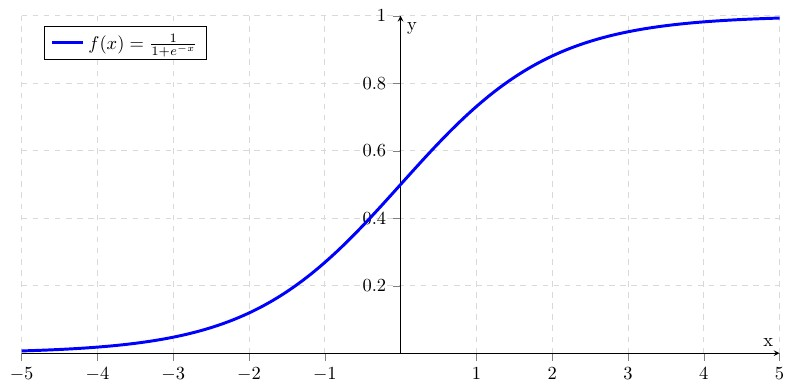
\includegraphics[width=0.4\textwidth]{Logistic-curve.jpeg}
\caption{\label{fig:SigmoidFunc}Sigmoid function}
\end{figure}

  \item Tanh function
\begin{equation}\label{eq:TanhFunc}
f(x) = \frac{e^{x}-e^{-x}}{e^{x}+e^{-x}}
\end{equation}

\graphicspath{ {./Figures/} }
\begin{figure}[!htb]
\centering
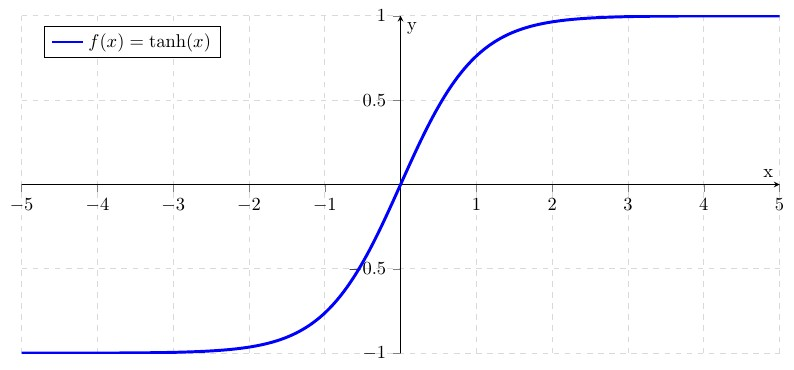
\includegraphics[width=0.4\textwidth]{tanh.jpeg}
\caption{\label{fig:TanhFunc}Tanh function}
\end{figure}
%  \item The third etc \ldots
\end{itemize}

We can also represent equation \ref{eq:FullEq} in vector notation, as in 
\begin{equation}\label{eq:UsedEq}
y = f(h) = f(w \cdot x)
\end{equation}
where $w$ and $x$ can be regarded as $n\times1$ dimensional column vectors, and $n$ is the dimension number of input data.
The term $w \cdot x$ in equation \ref{eq:UsedEq} constructs a $(n-1)$-dimension hyperplane which passes the origin. The hyperplane can be shifted by adding an parameter to equation \ref{eq:BasicEq}, for example
\begin{equation}\label{eq:WithBias}
y = f(h) = f(w \cdot x + b)
\end{equation}
We can have the same effect by putting a constant value $1$ and increasing the size of $x$ and $w$ by one. The extra weight $w$ with fixed value 1 is called \textit{bias weight}. It is adaptive like other weights and provides flexibility to hyperplane. Then we get:
\begin{equation}\label{eq:finalEq}
y = f(h) = f(\sum_{i=0}^{n}w_{i}x_{i})
\end{equation}
The aim of learning is to find a set of weights $w_{i}$ so that:
\begin{align*}
y = f(\sum_{i=0}^{n}w_{i}x_{i}) = 1  & \quad x \in Class A\\
y = f(\sum_{i=0}^{n}w_{i}x_{i}) = 0  & \quad x \in Class B
\end{align*}

The single layer neural network classifier is simple to implement, while it can only support a linear decision boundary. We can build a simple neural network to acquire intuition behind the mathematical theory. The network has no bias and one neuron which means it has one weight, say $w_{1}$. We implement a logistic sigmoid activation function on the multiply of input data and weight $w_{1}$. Therefore, the network can map the input data $a_0$ onto an output $a_{out}$ based on the function
\begin{equation}\label{eq:1LayerExample}
a_{out} = f(a_{0}w_{1})
\end{equation}
where $f()$ is the logistic function. Supposing that an input data $1$ maps to an output data $1$, we can compute the value of the error function for each possible value of $w_{1}$. Feeding value of $w_{1}$ in range $(-10,10)$, we can plot error surface in figure \ref{fig:1LayerErrorSurface}.
\graphicspath{ {./Figures/} }
\begin{figure}[!htb]
\centering
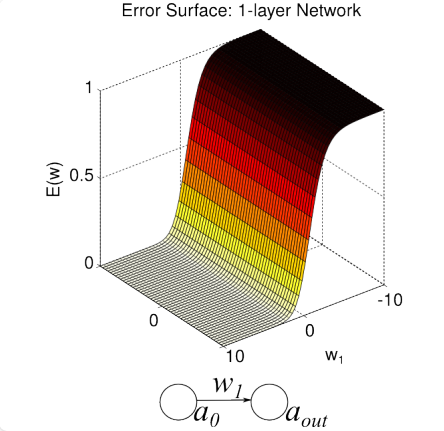
\includegraphics[width=0.4\textwidth]{1LayerErrorSurface.png}
\caption{\label{fig:1LayerErrorSurface}The error surface for a single layer neural network \citep{ErrorFigure1}.}
\end{figure}

The single layer neural network has a decision boundary which is linear. However, it is clear this is a very limited class of decision boundary. It can be illustrated by two types of datasets in figure \ref{fig:1Layer2datasets} .
\graphicspath{ {./Figures/} }
\begin{figure}[!htb]
\centering     %%% not \center
\subfigure{\label{fig:a}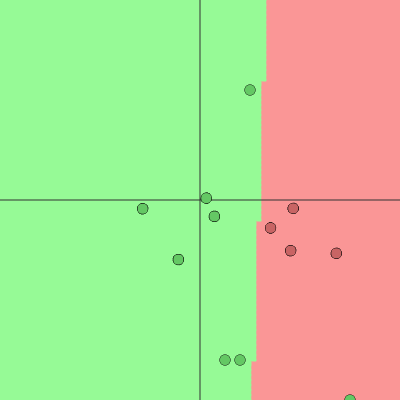
\includegraphics[width=0.4\textwidth]{SingleLayerSimpleData}}
\subfigure{\label{fig:b}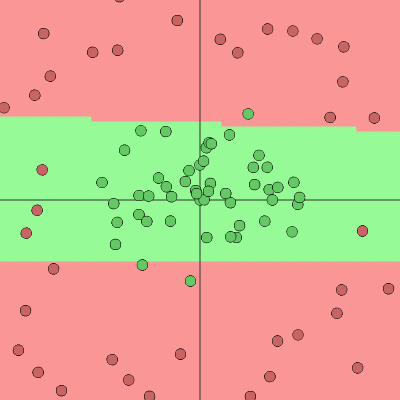
\includegraphics[width=0.4\textwidth]{SingleLayerCircleData}}
\caption{\label{fig:1Layer2datasets}Two types of dataset. The left one can be separated by a single layer neural network. The right one cannot be separated by a single neural network. Generated from \citep{GenerateNN}.}
\end{figure}

\section{Multi-Layer Networks}

Single layer networks have some important limitation in terms of representing range of functions. We are seeking to learn the nonlinearity as the linear discriminant. To improve the representation capability, we can stack layers network. This is the approach of multi-layer neural networks. multi-layer neural networks implement linear discriminants via mapping the input data to a nonlinear space. They can use fairly simple algorithms to learn the form of the nonlinearity from the training data.

In the thesis, we limit multi-layer neural networks in the subset of feedforward networks. Feedforward neural networks can provide a general mechanism for representing nonlinear functional mapping between a set of input data and a set of labels. The figure \ref{fig:ffnet} is a feedforward neural network having two layers of adaptive weights.

\begin{figure}[!htb]
\centering
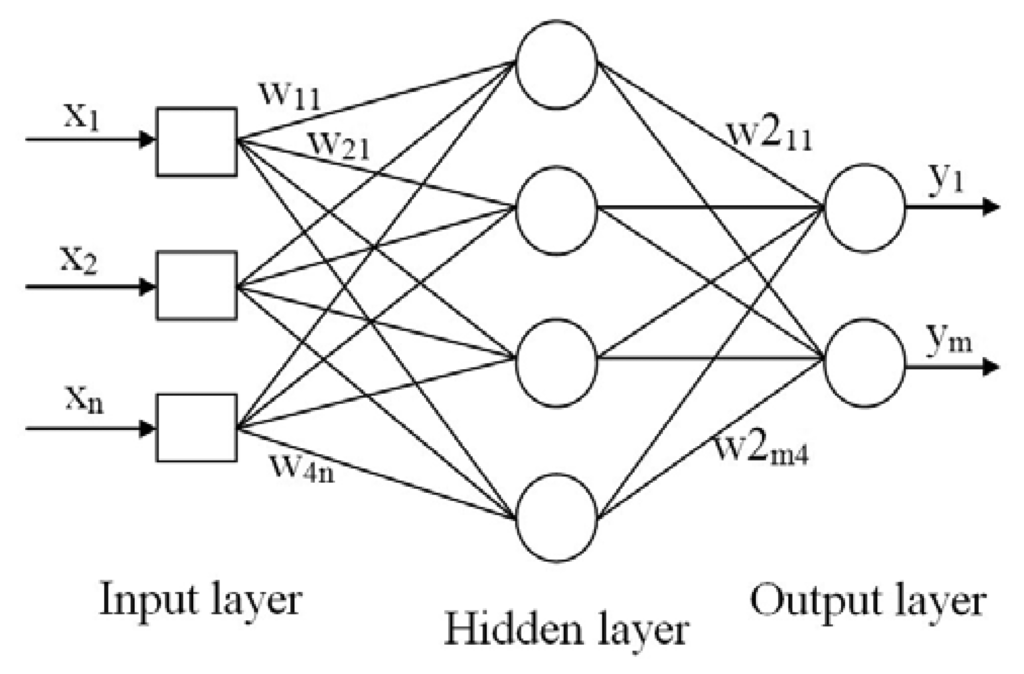
\includegraphics[width=0.8\textwidth]{Figure2-2.png}
\caption{\label{fig:ffnet}Diagram of a feedforward neural network \citep{zainal2013oil}.}
\end{figure}

In the example, the middle column perceptrons act as hidden neurons. The network has $n$ inputs, $4$ hidden neurons and $m$ output neurons. The network diagram represents the function in the form
\begin{equation}\label{eq:ffEq}
y_{m} = \hat{f}\Big(\sum_{j=0}^{m}w_{j4}^{(2)}f\big(\sum_{i=0}^{n}w_{4i}^{(1)}x_{i}\big)\Big)
\end{equation}
In equation \ref{eq:ffEq}, the outer activation function could be different with the inner one.

There are some choices for activation functions, the sigmoid and the tanh functions are related and continuous activation functions. The logistic function, also named the sigmoid function, can be represented as 
\begin{equation}\label{eq:sigmoid}
f(x) = \frac{1}{1+e^{-x}}
\end{equation}
Its outputs lie in the range $(0,1)$. We can do a linear transformation $\hat{x}=x/2$ on the input data and a linear transformation $\hat{y}=2y-1$ on the output. Then we can get an equivalent activation function tanh which can be represented:
\begin{equation}\label{eq:tanh}
f(x) = tanh(x) = \frac{e^{x}-e^{-x}}{e^{x}+e^{-x}}
\end{equation}

The three layers neural network is capable of approximating any function with enough hidden neurons, which means the network with two layers of weights and the sigmoid function can provide a high degree of accuracy in classification problems. 

Again, we can use a simple example to illustrate the power of the multi-layer neural network. In this example, we have one input, one hidden neuron and one output. There is no bias in the input layer and hidden layer. There are two weights existing in the network, say $(w_{1}, w_{2})$, and the output can be calculated via
\begin{equation}\label{eq:2LayerExample}
a_{out} = f(f(a_{0}w_{1})w_{2})
\end{equation}
where $f()$ is the sigmoid function. With varying $w_{1}$ and $w_{2}$, the error surface can be represented in figure \ref{fig:2LayerErrorSurface}.
\graphicspath{ {./Figures/} }
\begin{figure}[!htb]
\centering
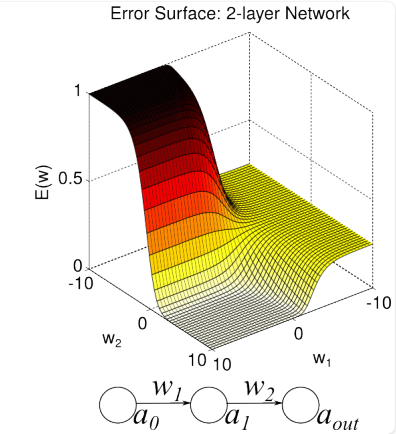
\includegraphics[width=0.4\textwidth]{2LayerErrorSurface.png}
\caption{\label{fig:2LayerErrorSurface}The error surface for a multi-layer neural network \citep{ErrorFigure1}.}
\end{figure}
And the samples which cannot be separated by the single-layer neural network can be done by a multi-layer neural network.
\graphicspath{ {./Figures/} }
\begin{figure}[!htb]
\centering
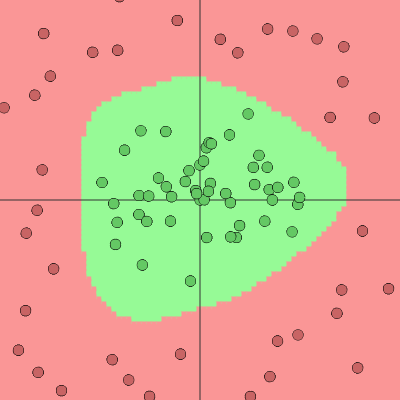
\includegraphics[width=0.4\textwidth]{MultiLayerCircleData.png}
\caption{\label{fig:MultiLayerErrorSurface}A multi-layer neural network can separate a complicated dataset. Generated from \citep{GenerateNN}.}
\end{figure}

\section{Stochastic Gradient Descent (SGD)}

Because the weight space in neural networks is continuous, training can reach the optimal weights value through optimization algorithms, which means minimising loss value of function
\begin{equation}\label{eq:LossMin}
L(f_{w}) = \sum L(y, f_{w}(x))
\end{equation}
Gradient descent is a first-order optimisation algorithm which starts from a random point, and then finds a nearby minimum point. It can converge on a minimum possible loss.

The SGD is a subtype of gradient descent. It only considers a single training point and moves to a nearby point based on
\begin{equation}\label{eq:SGDUpdate}
w = w - \eta  \Delta L(w) = w - \eta \sum_{i=1}^{n} \Delta L_{i}(w)
\end{equation}
where $\eta$ is the learning rate and $L_{i}(w)$ is the value of the loss function at the $i^{th}$ sample. The Robbins-Siegmund theorem \citep{robbins1985convergence} provides the approaches to almost surely convergence to a global minimum under relatively mild assumptions, moreover, it is fast and effective in practice.

\section{Backpropagation}

Multi-layer neural networks can represent mapping from the input data to the output classes. How to learn a suitable mapping method from the training dataset? And there is no explicit mapping between the outputs and the hidden neurons. This will be resolved by a popular learning algorithm, backpropagation.

Because networks have differentiable activation functions, the activation of the output neurons can be propagated to the hidden neurons with respect to weights and bias. If we have an error function, we can evaluate derivatives of the error and update the weights to minimise the error function via some optimization methods.

Backpropagation can be applied to find the derivatives of an error function related to the weights and bias in the network via two stages. First, the derivatives of the error functions, for instance sum-of-squares and Jacobian, with respect to the weights must be evaluated. Second, a variety of optimisation schemes can be implemented to compute the adjustment of weights based on derivatives. After passing data through the network, we can get the output result. It updates weight changes based on the grandient descent. Suppose the network has $i$ inputs, $h$ hidden neurons and $k$ outputs. The update equation can be represented: 
\begin{equation}\label{eq:UpdateWeights}
w(j+1) = w(j) + \Delta w(j)
\end{equation}
where $\Delta w(j)$ defined: 
\begin{equation}\label{eq:DeltaWeights}
\Delta w(j) = -\eta \frac{\partial E}{\partial w}
\end{equation}

For the hidden to output layer weights
\begin{equation}\label{eq:h2oBP}
\Delta w(jk) = -\eta \frac{\partial E}{\partial w_{jk}} = -\eta \delta_{k}y_{j}
\end{equation}
where $$\delta_{k} = \frac{\partial E}{\partial a_{k}} = (y_{k} - t_{k})y_{k}(1 - y_{k})$$

For the hidden layer weights
\begin{equation}\label{eq:hiddenBP}
\Delta w(ij) = -\eta \frac{\partial E}{\partial w_{ij}} = -\eta \delta_{j}y_{i}
\end{equation}
where $$\delta_{j} = \frac{\partial E}{\partial a_{j}} = \displaystyle\sum_{k} \delta_{k}w_{jk}y_{j}(1 - y_{j})$$

The $\delta_{j}$ of a hidden neuron is based on the $\delta_{k}$ of the output neurons to which it links. To minimise the error function $E$ with the gradient descent, it needs the backwards propagation of errors.

\subsection{Training protocols}

In supervised learning, we have training dataset which are data with labels. We can use the neural networks to find the output of the training data and adjust the weights to optimal values. There are mainly  three types of training protocols, stochastic, batch and online training. In stochastic training, we randomly choose samples from the training dataset and update weights every time, depending on the output of the network. In batch training, we use some samples and pass them through the network, and then update weights. In online training, each sample of the training dataset is used once and weights are updated each time. We usually represent one time of passing all training dataset through neural networks as one epoch.

It is worth noting batch learning. In large scale applications, the training dataset can be over millions of samples. It is time consuming to compute the loss function over all training datasets in order to update weights once. It is a practical approach that computes the gradient over a batch of training datasets. Does it have harmful effects on generalisation? It depends on the correlations among the training dataset. Consider there are more than one million images in the ImageNet dataset which is made up of only 1000 categories. If the images in a batch are selected evenly from each category, the gradient from the batch is a good enough approximation of the gradient of the full training dataset. Therefore, batch learning leads to faster convergence by evaluating the batch gradients to update weights frequently.

\section{Overfitting and Regularization}

Overfitting is a common phenomenon that a model has high performance on the training dataset, but is poor on the testing dataset in classification tasks. Thus, a classification problem with two classes and two input variables, (left figure in \ref{fig:OverfittingExample}), shows decent decision boundaries. With increasing complexity of the model, the decision boundaries become more complex and fit the training dataset extremely well.
\graphicspath{ {./Figures/} }
\begin{figure}[!htb]
\centering
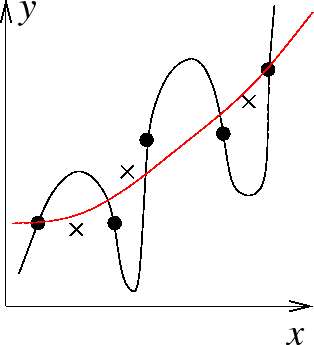
\includegraphics[width=0.8\textwidth]{overfitting.png}
\caption{\label{fig:OverfittingExample}Overfitting example, the left one has a decent generalisation performance and the right one is overfitting \citep{OverfittingFigure}.}
\end{figure}
From the example in figure \ref{fig:OverfittingExample}, it is clear that a model, whose complexity is neither too small nor too large, has the best generalisation performance. 

In order to find the optimal complexity of the neural network, there are mainly two approaches. One is to change the adaptive parameters, like neuron numbers in hidden layers. This is named structural stabilisation. It can be approached from two directions. We can start from a small network and increase the layer number or neuron number in the training process and arrive at an effective neural network architecture. The other one is to start from a large network and prune out layers or neurons in the training process to achieve the optimal network. Another fundamental basic method to control the complexity of a model is to use regularisation which includes adding a penalty term in the error function. The degree of regularisation can be adjusted by scaling the term via a multiplicative parameter.

Regularization helps to smooth decision boundary surface by introducing a penalty term $\Omega$ to the error function
\begin{equation}\label{eq:Regularization}
\hat{E} = E + \lambda\Omega
\end{equation}
where $E$ is the standard error function, the $\lambda$ adjustment and the extent of the penalty $\Omega$ effects on the solution. The task of the learning is to minimize the total error function $\hat{E}$. It needs to compute the derivatives of $\Omega$ with respect to the weights efficiently. A model, which has high accuracy in the training dataset, has a small value for $E$. At the same time, the smooth error surface of neural networks give a small value for $\Omega$.

A number of regularisers have been performed in applications, like weight decay, early stopping, training with noise, weight sharing etc..

\subsection{Weight Decay}

In order to smooth the decision boundary surface, weight values should be small. The weight decay regularizer can be represented:
\begin{equation}\label{eq:WeightDcay}
\Omega = \frac{1}{2} \sum_i w_{i}^2
\end{equation}
where the sum includes all weights and bias. Weight decay of this form leads to major improvements in empirical generalisation \citep{hinton1987learning}. Intuitively, in equation \ref{eq:WeightDcay}, the smaller the weights are, the better the regulariser is. Usually, the derivatives of the total error function with respect to the weight are used to train the neural network. The network is trained by gradient descent in the continuous time limit. The weights will evolve with time $t$
\begin{equation}\label{eq:WeightDecayTime}
\frac{w}{t} = -\eta\nabla E = -\eta\lambda w
\end{equation}
where $\eta$ is the learning rate. And the equation has solution
\begin{equation}\label{eq:WeightDecaySolution}
w(t) = w(0)exp(-\eta\lambda t)
\end{equation}
and the exponential function reduces weights to zero quickly. Weight decay is also named L2 regularisation.

\subsection{Dropout}

Neural networks with deep layers and a large amount of neurons is a powerful learning machine. However, the more parameters the network has, the easier it is overfitting. Recently, dropout \citep{srivastava2014dropout} is a simple and extremely effective regularisation technique which complements the other methods. At the training process, random neurons are selected with some probability $p$ to update their associated weights, and the others are inactive. In other words, only a reduced network is trained, based on the input data at the training stage. 
\graphicspath{ {./Figures/} }
\begin{figure}[!htb]
\centering
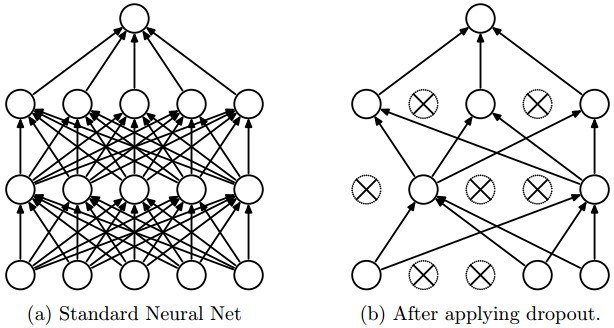
\includegraphics[width=0.8\textwidth]{dropout.jpeg}
\caption{\label{fig:Dropout}Illustration of dropout \citep{srivastava2014dropout}.}
\end{figure}
At the testing process, there is no dropout applied and all neurons are active. The dropout method is replaced by performing a scaling of layer outputs by the same probability $p$. This method can keep the outputs of neurons to be the same in both training and testing process. For example, if a neuron has $p$ probability to be dropped out in the training process, the neuron should give an output $l$ without dropout in the testing stage. Then we should apply $(p\ast l + (1 - p)\ast 0)$ on the output, because the output has $(1-p)$ probability to be $0$.

\section{Softmax Classifier}

The softmax function, also named normalised exponential, is a generalisation of the logistic function which squeezes a $d$ dimensional arbitrary real values vector to a $d$ dimensional vector of real values in the range $(0,1)$ that add up to 1. Because the softmax function is the gradient log normaliser of categorical probability distribution, it can be used in probabilistic multiclass classification problems.

The softmax function derives from log linear models and interprets the weights in terms of convenient odds ratios. It can constrain the input values of the final layer to be positive and sum of them to be $1$.

The softmax layer begins the same way as the normal layer which forms the weighted inputs $z^L_j = \sum_{k} w^L_{jk} x^{L-1}_k + b^L_j$ where $L$ is the layer number, $k$ is the input data number and $j$ is the output neuron number. It, then, implements a softmax function to the $z^L_j$ and activates the $j$ output neuron:
\begin{equation}\label{eq:SoftmaxActivation}
f_j(z) = \frac{e^{z_j}}{\sum_k e^{z_k}}
\end{equation}
The equation \ref{eq:SoftmaxActivation} implies that the output values are all positive and the sum of all values $\sum_k a_k$ is $1$.

The softmax classifier can be used to handle a multiclass classification. For a training dataset $(x_{1}, y_{1}), \ldots, (x_{m}, y_{m}), y_{i} \in \{1, 2, \ldots, K\} $ of $m$ labelled examples, the label $y$ can have $K$ different values.

To an unseen sample $x$, we will use a hypothesis to estimate the probability $P(y=k | x)$ for each value $k = 1, \ldots, K$. For example, we want to compute the probability of the class label on each of $K$ different possible values. The neural network will then output a $K$ dimensional vector which represents $K$ estimated probabilities. 
%\begin{equation}\label{eq:SoftmaxPostPro}
\begin{align}
h_{W}(x) =
\begin{bmatrix}
P(y = 1 | x; W) \\
P(y = 2 | x; W) \\
\vdots \\
P(y = K | x; W)
\end{bmatrix}
=
\frac{1}{ \sum_{j=1}^{K}{\exp(W^{(j)\top} x) }}
\begin{bmatrix}
\exp(W^{(1)\top} x ) \\
\exp(W^{(2)\top} x ) \\
\vdots \\
\exp(W^{(K)\top} x ) \\
\end{bmatrix}
\end{align}
%\end{equation}
Where $W^{j}$ are the weights of the model and the normalised distribution ensures that the sum is one.

On the one hand, the cross entropy can be used to interpret the softmax classifier. The cross entropy between actual  distribution $p$ and a predicted distribution $q$ is represented as
\begin{equation}\label{eq:CrossEntropyDiff}
H(p,q) = - \sum_x p(x) \log q(x)
\end{equation}
Hence, the task of the softmax classifier is to minimise the cross entropy between the actual distribution and the predicted distribution. 

On the other hand, the softmax classifier can be interpreted in probability view. Given a sample $(x_i, y_i)$ and parameters $W$, we can compute the normalised probability:
\begin{equation}\label{eq:ProbInter}
P(y_i \mid x_i; W) = \frac{e^{f_{y_i}}}{\sum_j e^{f_j} }
\end{equation}
where $f_{y_i}$ is the score predicted by the model with weights $W$. Therefore the normalised probabilities are computed by exponentiating the values and dividing the sum of all values. We can minimise the negative log likelihood of the ground truth labels which can be regarded as performing the Max Likelihood Estimation(MLE). Aside from MLE, the Maximum a posteriori(MAP) can also be used to evaluate the performance of a model.

\subsection{Practical issues}

From a numerical view, the exponential computation is easy overflow. Thus, the output of the softmax function is not numerically stable through computing $e^{f_{y_i}}$ and $\sum_j e^{f_{y_j}}$ directly. The implementation requires a normalisation trick. It is mathematically equivalent to multiplying a constant $C$ with both the top and bottom of the fraction.
\begin{equation}\label{eq:SoftmaxTricks}
\frac{e^{f_{y_i}}}{\sum_j e^{f_j}}
= \frac{Ce^{f_{y_i}}}{C\sum_j e^{f_j}}
= \frac{e^{f_{y_i} + \log C}}{\sum_j e^{f_j + \log C}}
\end{equation}
where $C$ can be any positive value. The constant $C$ does not change the output value, but it can improve the numerical stability of the computation. An experienced choice of $C$ is to set $\log C = -\max f_j$, and it can shift the vector $f$ to preserve the highest value as $0$.

\subsection{Error function}
An error function is used to evaluate the performance of a model. We will generate an error function for softmax regression. An indicator function, $I\{\cdot\}$, is introduced to represent the accuracy for each label. If the predicted result corresponds to the actual label, say $y^{(i)} = k$, the indicator function returns $1$, otherwise $0$. The error function will be defined:
\begin{equation}\label{eq:LogLossFunc}
L(W) = - \left[ \sum_{i=1}^{m} \sum_{k=1}^{K}  I\left\{y^{(i)} = k\right\} \log \frac{\exp(W^{(k)\top} x^{(i)})}{\sum_{j=1}^K \exp(W^{(j)\top} x^{(i)})}\right]
\end{equation}
where this generates the logistic regression error function
\begin{align}\label{eq:LogRegLossFunc}
L(W) &= - \left[ \sum_{i=1}^m   (1-y^{(i)}) \log (1-h_W(x^{(i)})) + y^{(i)} \log h_W(x^{(i)}) \right] \\
&= - \left[ \sum_{i=1}^{m} \sum_{k=0}^{1} 1\left\{y^{(i)} = k\right\} \log P(y^{(i)} = k | x^{(i)} ; W) \right]
\end{align}
Similar to the logistic regression error function, the softmax error function sums over the predicted different $K$ values of the classes. In the softmax regression, the posterior probability distribution can be represented:
\begin{equation}\label{eq:PostProbDis}
P(y^{(i)} = k | x^{(i)} ; W) = \frac{\exp(W^{(k)\top} x^{(i)})}{\sum_{j=1}^K \exp(W^{(j)\top} x^{(i)}) }
\end{equation}
It is not easy to solve equation \ref{eq:LogRegLossFunc}. Usually an optimisation algorithm can approximate the optimal value. Taking derivative with respect to weights, we can get the entire gradient 
\begin{equation}\label{eq:PartDer}
\nabla_{W^{(k)}} L(W) = - \sum_{i=1}^{m}{ \left[ x^{(i)} \left( 1\{ y^{(i)} = k\}  - P(y^{(i)} = k | x^{(i)}; W) \right) \right]  }
\end{equation}
We can take partial derivative of $L(W)$ with respect to the $j$th element of $W^{(k)}$.

\section{Convolutional Neural Networks (CNN)}

Convolutional Neural Networks \citep{lecun1998gradient} are widely applied in image understanding and achieve top rank in an image classification competetion \citep{krizhevsky2012imagenet}. Compared to regular neural networks, CNN architecture assumes that the inputs are images and pixels are related in region. Regular neural networks fully connect layers and the method causes expensive computation.

CNN architecture has neurons arranged in 3 dimensions, say width, height and depth. For example, there is an image which has dimensions $32\times 32\times 3$. The neurons in a layer will connect to a customised region of the previous layer. Moreover, the final output layer has dimensions $1\times 1\times d$, where $d$ is the number of classes. The dimensions are reduced from $3072$ to $d$. The output is a single vector of class scores.

\graphicspath{ {./Figures/} }
\begin{figure}[!htb]
\centering
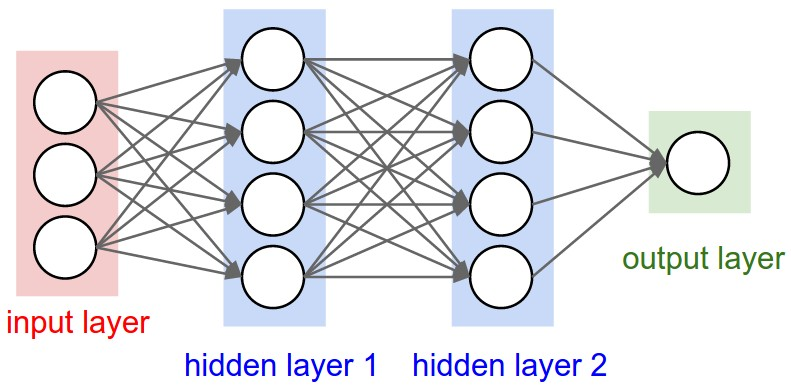
\includegraphics[width=0.4\textwidth]{neural_net2.jpeg}
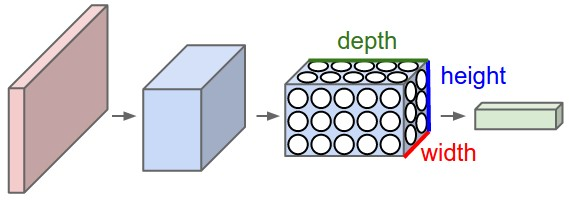
\includegraphics[width=0.4\textwidth]{cnn.jpeg}
\caption{\label{fig:compareCNNandFC}The left is a fully connect regular neural network. The right is a CNN in 3 dimensions \citep{CNNDiagram}.}
\end{figure}

\subsection{Layers in CNN}
CNNs have three main types of layers, convolutional layer, pooling layer and fully connected layer. Every layer transforms the input to the output via a differentiable function. 
\begin{enumerate}
  \item Convolutional Layer
  \item ReLU Layer
  \item Pooling Layer
  \item Fully Connected Layer
\end{enumerate}
Following layer by layer, CNN transforms an image from a set of pixel values to the final class scores.

\textbf{Convolutional Layer} is the key component of CNN and its output can be represented as neurons shaped in 3D volume. A set of learning filters make up the convoultional layer's parameters. Although the size of filter is flexible, it is usually small. During the feedforward process, each filter slides across the input volume and produces a $2$-dimensional feature map. In each slide, the input and the filter have a dot product computation. If there are some specific feature at some spatial position, they can be learnt by filters.

Local connectivity is the key properties of the CNN. Regular neural networks use fully connected layers. That is unaffordable for images, even with high capability hardware. Instead, each neuron connects a local region of the input only. There are two main benefits from local connectivity. One is reducing parameters significantly and controlling overfitting. The other one is from a key image property. Pixels are strongly correlated with nearby pixels. This can be regarded as a local receptive field which can retrieve information from subregions of the image.

\graphicspath{ {./Figures/} }
\begin{wrapfigure}{r}{0.5\textwidth}
  \begin{center}
    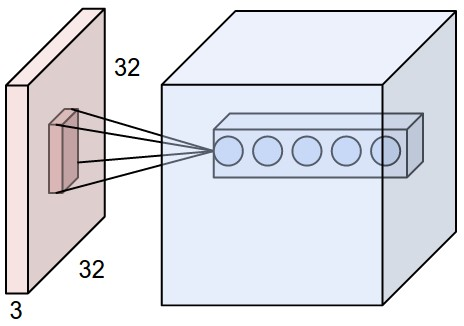
\includegraphics[width=0.48\textwidth]{depthcol.jpeg}
  \end{center}
  \caption{Diagram for depth in a convolutional layer \citep{CNNDiagram}.}
\end{wrapfigure}
To control the output volume arrangement, three parameters are introduced. They are depth, stride and zero-padding. In convolutional layer, depth controls the number of neurons which connect the same subregion of the input volume. All the neurons learn the different features from the input volume. For example, the neurons along the depth in the convolutional layer after the input data layer can activate existence of various edges, colour, etc.. Stride is another parameter which controls the spatial position of the nearby depth column of neurons. The smaller the stride is, the more overlapping receptive fields are shared by the nearby columns. Last, zero-padding on border makes output volume to keep the same dimension with the input volume.

A scheme, named parameter sharing, is implemented in convolutional layer to limit the number of parameters. The scheme suppose that a filter, which is helpful to compute at some spatial positions, should be helpful to compute another position.

\textbf{ReLU Layer} is the abbreviation of Rectified Linear Units. The neurons in the layer operate the non-saturating activation function $f(x) = max(0,x)$ over the result of dot product in convolutional layers. The layer increases non linearity to network without losing the receptive fields of convolutional layers.

\textbf{Pooling Layer} is a mechanism of downsampling. It is usually appended after the convolutional layer to progressively decrease the spatial size of the feature map. It leads to decrease network parameters and makes the neurons in pooling layer to be relatively insensitive to small shifts of the image.

\textbf{Fully Connected Layer} takes feature maps, which have high level representation, from previous layers. Its difference with convolutional layer is that it connects to all neurons in previous layer instead of a receptive field only.

\section{Spatial Pyramid Matching (SPM)}

The spatial pyramid matching \citep{lazebnik2006beyond} is used to classify high-level semantic attributes, based on low-level features. The method subdivides an image in several different levels of resolution and counts features falling in each spatial bin. It extends bags of features and derives spatial information from the image.
\graphicspath{ {./Figures/} }
\begin{figure}[!htb]
\centering
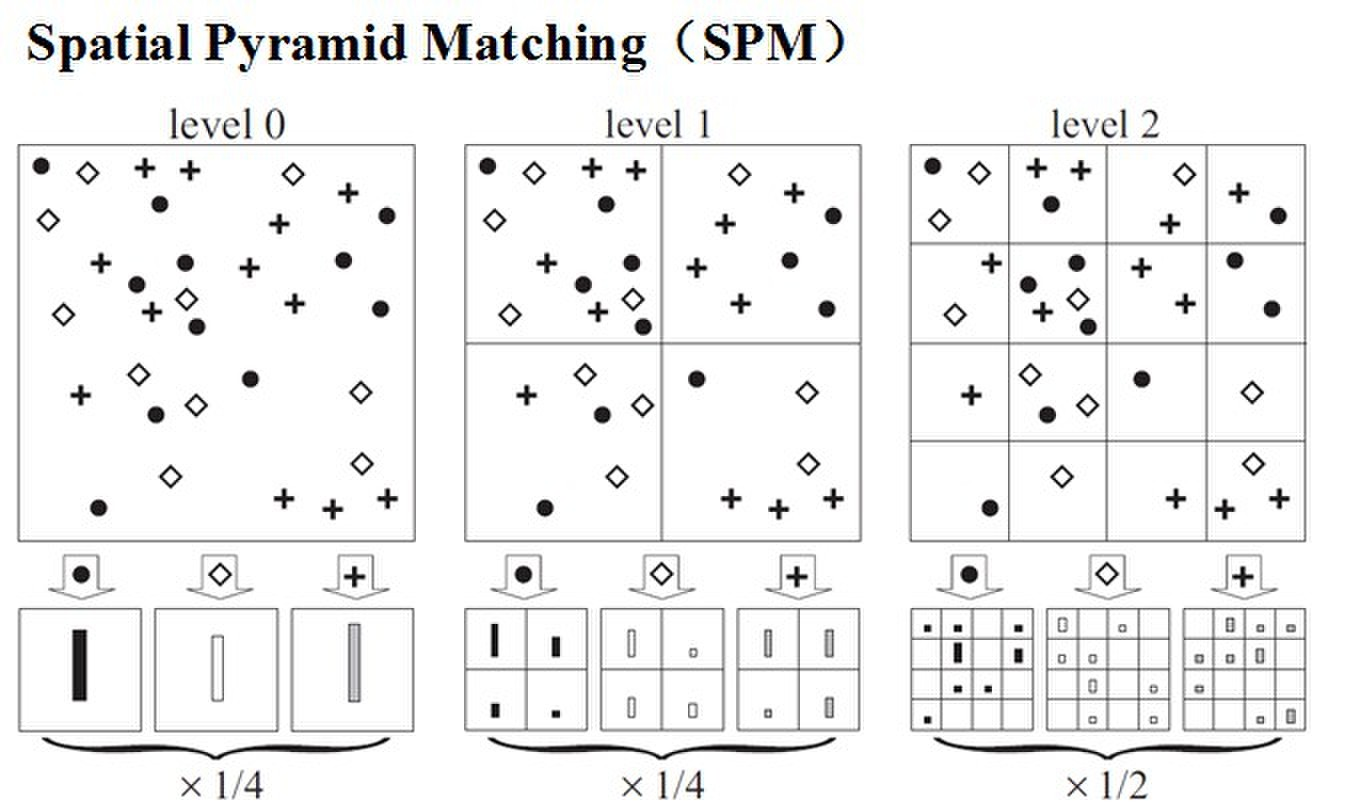
\includegraphics[width=0.8\textwidth]{spm.jpg}
\caption{\label{fig:SpatialPyramidMatching}Diagram of the Spatial Pyramid Matching \citep{lazebnik2006beyond}.}
\end{figure}

Let two sets of vectors $X$ and $Y$ be in a $d$-dimensional feature space. The SPM is used to find the approximate correspondence between them. In brief, the SPM places a chain of grids over the feature space and takes the sum of number of matches occuring at each level of resolution. The points falling into the same grid are matched and the match points in finer resolutions have higher weights. Specifically, a chain of grids at resolutions $0,\dotso,L$, have $2^0,\dotso,2^L$ cells respectively. $H_{X}^l$ and $H_{Y}^l$ are the histograms of $X$ and $Y$ at the $l$ resolution, so that the number of points in the $i$th cell from $X$ and $Y$ can be represented as $H_{X}^l(i)$ and $H_{Y}^l(i)$. The histogram intersection function denotes the number of matches at level $l$
\begin{equation}\label{eq:HistInterFunc}
I(H_{X}^l, H_{Y}^l) = \sum_{i=1}^D min(H_{X}^l(i), H_{Y}^l(i))
\end{equation}

Because the match points found in the $l$ level include the match points found in the finer level $l+1$, the number of new match points at level $l$ is $I^l - I^{l+1}$. The weight assigned to level $l$ is $\frac{1}{2^{L-l}}$. Putting all together, the pyramid match kernel can be represented:
\begin{eqnarray}\label{eq:PyramidChanMatchKernel}
  K^L(X,Y) & = & I^L + \sum_{l=0}^{L-1} \frac{1}{2^{L-l}}(I^l-I^{l+1})\\
 & = & \frac{1}{2^L}I^0 + \sum_{l=1}^{L}\frac{1}{2^{L-l+1}}I^l
\end{eqnarray}
We perform the SPM in a $2$-dimensional image space and apply standard vector quantisation in the feature space. All feature vectors are quantised into $M$ discrete types and only the same type of features match to one another. Two sets of $2$-dimensional vectors, $X_m$ and $Y_m$, represent the coordinate of the features of type $m$ in the individual image. The match kernel of two images is the sum of total channel kernels
\begin{eqnarray}\label{eq:PyramidMatchKernel}
  K^L(X,Y) = \sum_{m=1}^{M} K^L(X_m, Y_m)
\end{eqnarray}

\section{Transfer Learning}

In the literature on machine learning, the transfer learning \citep{pan2010survey} focuses on storing knowledge from one domain and applying it to a related problem. In other words, the relevant knowledge, learned from previous tasks, can be applied to new tasks. The closer a new job relates to previous knowledge, the more easily it can be solved. In contrast, other machine learning methods solve problems independently. 

The transfer learning has three benefits. One is saving time of preprocessing data. Collecting and processing raw data are time consuming and expensive in each task. It can reduce volume of required data significantly, based on existing knowledge which is extracted from previous learning tasks. The other one is saving time of learning the model from scratch up. Usually, training a model from scratch up is time consuming. The transfer learning can save a lot of time. The last one is to avoid the risk of overfitting. With insufficient training data, a complicated model is easy to overfitting. The transfer learning method can control overfitting because of existing knowledge.

\graphicspath{ {./Figures/} }
\begin{figure}[!htb]
\centering
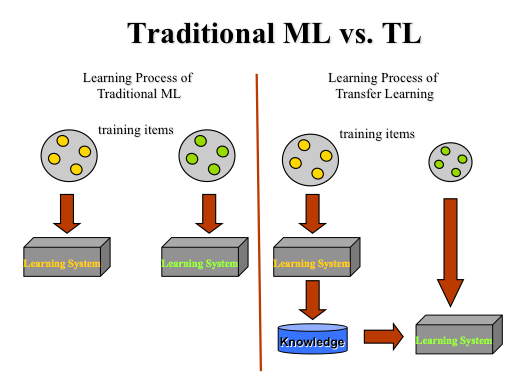
\includegraphics[width=0.8\textwidth]{MLvsTL.png}
\caption{\label{fig:TransferLearning}The left is traditional machine learning method. The right is transfer learning \citep{TransferlearningDiagram}.}
\end{figure}

A domain can be represented
\begin{equation}\label{eq:TransLearning}
D = \{ X, P(X) \}
\end{equation}
where $X$ is the feature space and $P(X)$ is the marginal probability distribution. 

In the transfer learning, there are two main challenges: 
\begin{enumerate}
  \item Which part of previous knowledge is useful to the new task?
  \item How to represent the existing knowledge in the new model?
\end{enumerate}
The first challenge arise, when we evaluate the relation between the previous knowledge and the current task. The correlated knowledge for the task can improve the performance of the model. Meanwhile, the unrelated and the negative correlated knowledge are useless, or even harmful for the task. After evaluating the useful knowledge, new learning algorithms should be developed to transfer the knowledge. This leads to the second challenge. Because knowledge can have different representations, the translation process must keep the accuracy and minimise the loss of knowledge. 